\section{Exchange}
Figure 1 shows a decision problem with three variables. There are $N!$ possible assignments of the variables, so when $N = 3$ there are $6$ possible assignments. The yellow circle shows an arbitrary starting assignment, and the arrows represents applying the 3-exchange and 2-exchange neighborhood functions. By following the arrows, we see that all possible assignments are reachable. The unique assignments are marked in red. The yellow starting point can be exchanged for any of the red circles, and all possible assignments will still be reachable from the initial assignment.

Now we have shown that applying 3-exchange and then 2-exchange to a decision problem with $3$ variables is complete.\\
\begin{figure}[h]
 \centering
 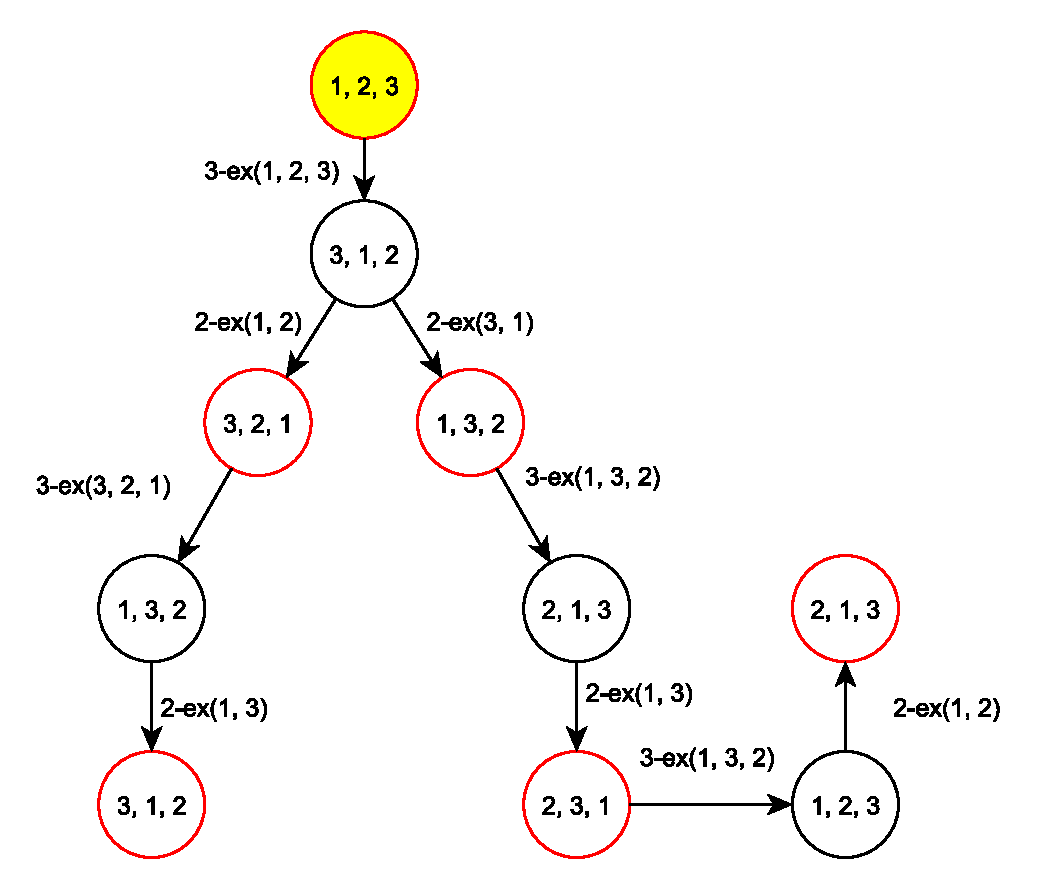
\includegraphics[width=12cm]{maingraph.pdf}
 \caption{3- and 2-exchange with 3 variables is complete}
 \label{figure:maingraph}
\end{figure}\\
\pagebreak
On figure 2 is a decision problem with $N$ variables, $-*$ is meant to show an infinite amount of variables. Figure 2 shows how it is possible swap any of the three first three variables with the fourth variable shown as $-$.

Now we have shown that a single variable can be moved to any position in as $N$ variable decision problem with 3-exchange and 2-exchange. Combined with the knowledge that any three variables can be placed in every possible assignment we can infer that a local search algorithm that uses 3-exchange followed by 2-exchange is complete.
\begin{figure}[h]
 \centering
 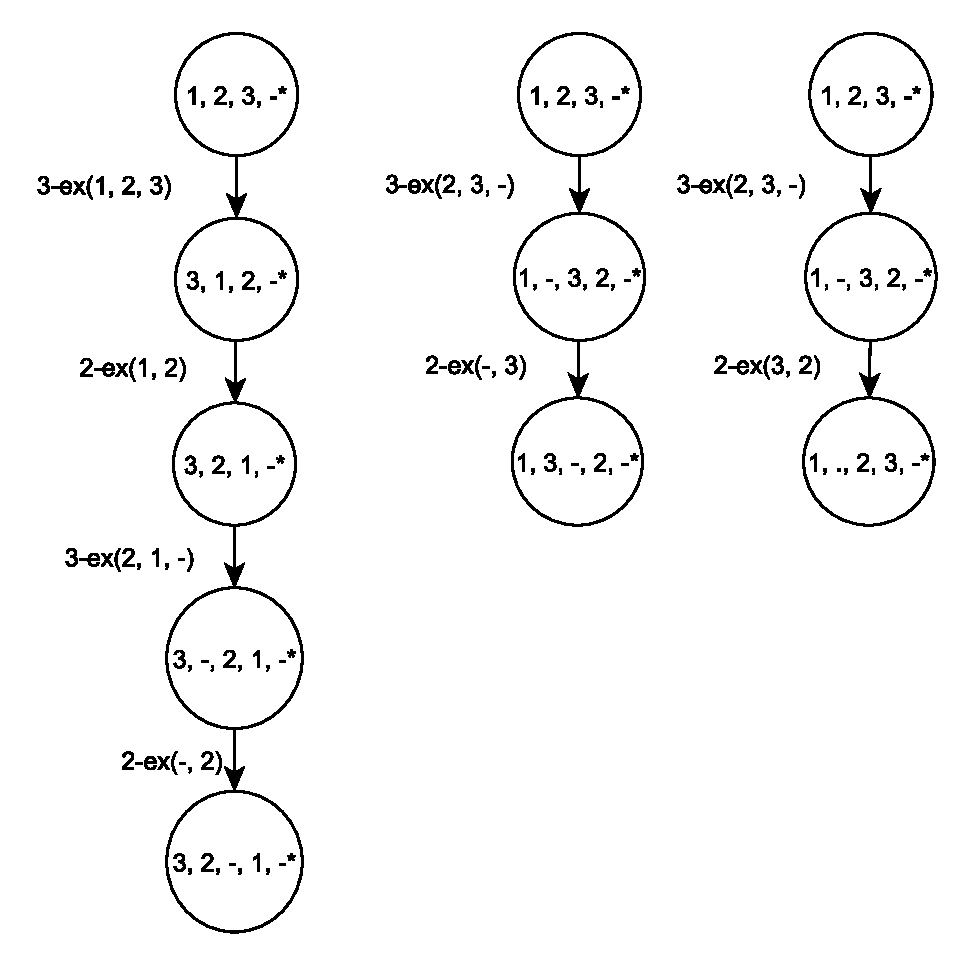
\includegraphics[width=12cm]{fig2.pdf}
 \caption{Varibles can be moved anywhere}
 \label{figure:fig2}
\end{figure}